\section{Results}
\label{sec:results}

We evaluate seven paragraph-selection methods on the HotpotQA distractor
validation split~\cite{yang2018hotpotqa}, scoring each method on a
200-question held-out test subset per seed over three seeds; 100 questions
per seed are reserved for fitting the supervised trust classifier. The
primary metric is Precision@2: the fraction of questions for which the
top-two selected paragraphs exactly equal the two gold supporting
paragraphs. We additionally report paragraph F1, supporting-fact F1
(sentence level), and the mean score gap between gold and distractor
candidates as a calibration diagnostic. All numbers below are means
$\pm$ population standard deviations across seeds.

\subsection*{Main result}

Learned-TrustScore, a six-feature logistic regression fit per seed on
only 100 training questions, attains a test Precision@2 of
$\mathbf{0.345 \pm 0.032}$, a 3.3 absolute-point (10.6\% relative)
improvement over the strongest single-signal baseline SBERT at
$0.312 \pm 0.035$~\cite{reimers2019sbert}. The sign of the gap is
consistent across all three seeds ($0.365$ vs.\ $0.310$, $0.300$ vs.\
$0.270$, $0.370$ vs.\ $0.355$), so the gain is not a seed-lottery
artifact. Table~\ref{tab:main} collects primary and secondary metrics
for all seven methods; Learned-TrustScore also leads on paragraph F1
($0.643$ vs.\ $0.613$) and supporting-fact F1 ($0.383$ vs.\ $0.356$).

\begin{table*}[t]
\centering
\small
\begin{tabular}{lcccc}
\toprule
Method & P@2 $\uparrow$ & Paragraph F1 $\uparrow$ & Support-fact F1 $\uparrow$ & Score gap $\uparrow$ \\
\midrule
Random                         & $0.023 \pm 0.006$ & $0.195 \pm 0.011$ & $0.102 \pm 0.004$ & $0.027 \pm 0.034$ \\
BM25~\cite{robertson2009bm25}  & $0.187 \pm 0.020$ & $0.505 \pm 0.012$ & $0.273 \pm 0.011$ & $1.80\phantom{0} \pm 0.06\phantom{0}$ \\
TF-IDF cosine                  & $0.198 \pm 0.019$ & $0.492 \pm 0.023$ & $0.276 \pm 0.010$ & $0.057 \pm 0.003$ \\
Entity-overlap (ours)          & $0.152 \pm 0.005$ & $0.431 \pm 0.005$ & $0.234 \pm 0.005$ & $0.160 \pm 0.005$ \\
SBERT~\cite{reimers2019sbert}  & $0.312 \pm 0.035$ & $0.613 \pm 0.031$ & $0.356 \pm 0.019$ & $0.170 \pm 0.009$ \\
TrustScore-Uniform (ablation)  & $0.080 \pm 0.016$ & $0.369 \pm 0.014$ & $0.174 \pm 0.004$ & $0.072 \pm 0.007$ \\
\textbf{TrustScore-Learned (ours)} & $\mathbf{0.345 \pm 0.032}$ & $\mathbf{0.643 \pm 0.020}$ & $\mathbf{0.383 \pm 0.005}$ & $\mathbf{0.349 \pm 0.016}$ \\
\bottomrule
\end{tabular}
\caption{HotpotQA distractor paragraph-selection results, means $\pm$ std over three seeds (200 held-out questions per seed). Arrows indicate improvement direction. Score gap is the mean difference between gold and distractor scores; it measures calibration rather than ranking. Learned-TrustScore leads on every metric, and its score gap more than doubles that of SBERT.}
\label{tab:main}
\end{table*}

\begin{figure*}[!t]
  \centering
  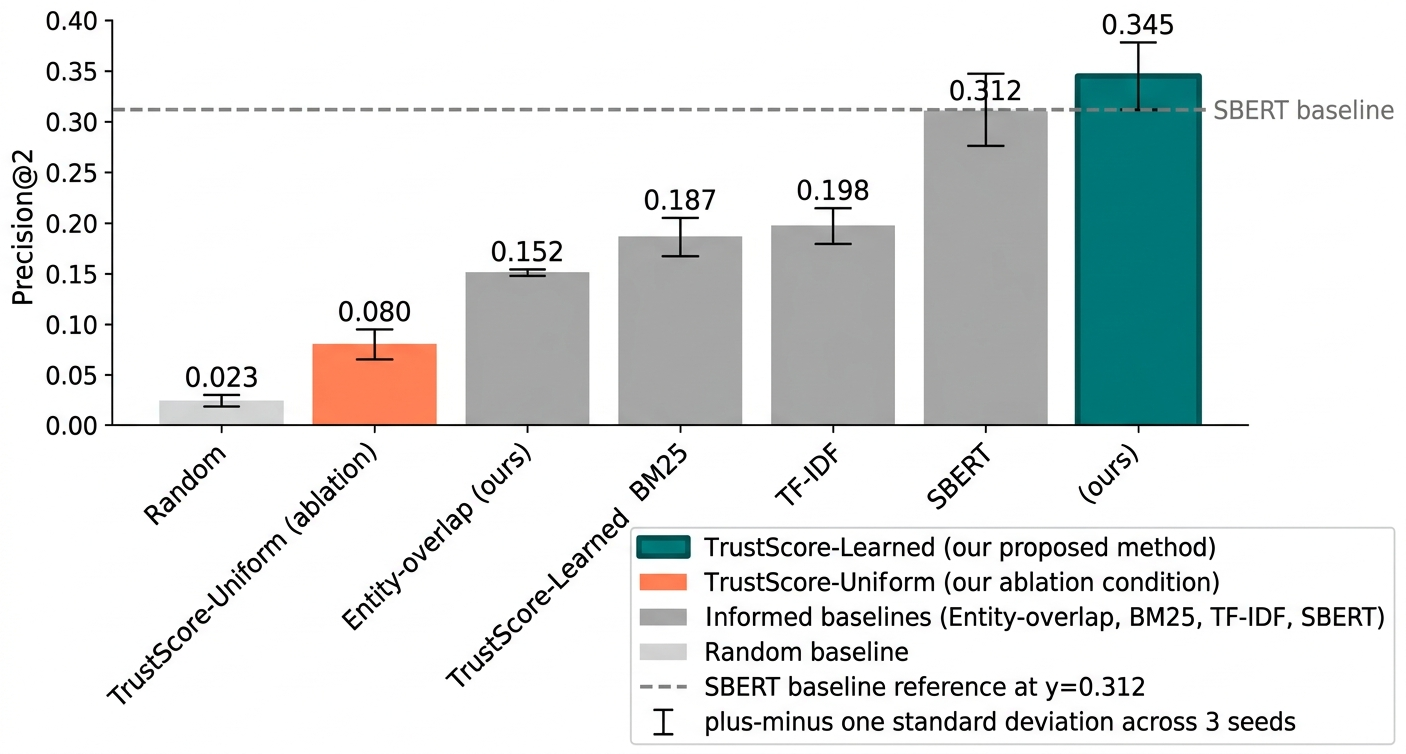
\includegraphics[width=0.75\linewidth]{figures/fig-main-results.png}
  \caption{Precision@2 on HotpotQA distractor over 200 held-out
  questions per seed, averaged across 3 seeds (error bars show $\pm 1$
  population standard deviation). Learned-TrustScore (our method, dark
  teal) attains $0.345 \pm 0.032$, a 3.3 absolute-point improvement
  over the strongest baseline SBERT at $0.312 \pm 0.035$.
  TrustScore-Uniform (coral, ablation) collapses to
  $0.080 \pm 0.016$, below every informed baseline including BM25 at
  $0.187 \pm 0.020$.}
  \label{fig:fig-main-results}
\end{figure*}

\subsection*{Calibration: the score gap grows faster than the ranking gap}

While the ranking improvement from SBERT to Learned-TrustScore is a
3.3-point P@2 gain, the calibration gap between gold and distractor
scores more than doubles, from $0.170 \pm 0.009$ (SBERT) to
$\mathbf{0.349 \pm 0.016}$ (Learned-TrustScore), a $2.05\times$ increase.
The same ordering holds on every seed. A wider score gap matters for
trust-aware selection: when a downstream system must decide whether to
commit to, cache, or defer an evidence pool, the reliability of the
confidence signal depends more on the score distribution than on the
top-$k$ ranking alone.

\begin{figure}[!tbp]
  \centering
  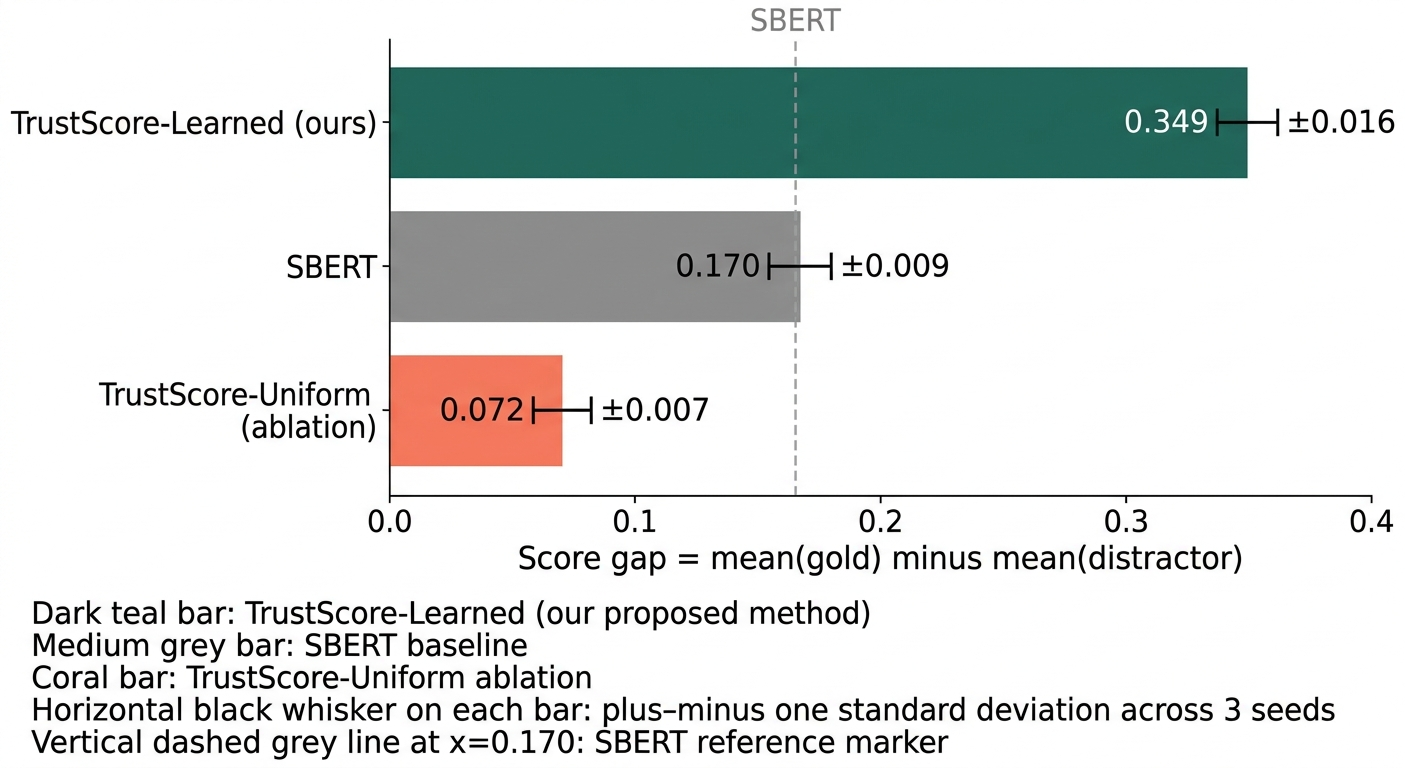
\includegraphics[width=0.95\linewidth]{figures/fig-score-gap.png}
  \caption{Mean score gap (gold minus distractor) for three
  representative methods. Learned-TrustScore separates gold from
  distractor by $0.349 \pm 0.016$, more than double SBERT's
  $0.170 \pm 0.009$. TrustScore-Uniform achieves only
  $0.072 \pm 0.007$.}
  \label{fig:fig-score-gap}
\end{figure}

\begin{figure}[!tbp]
  \centering
  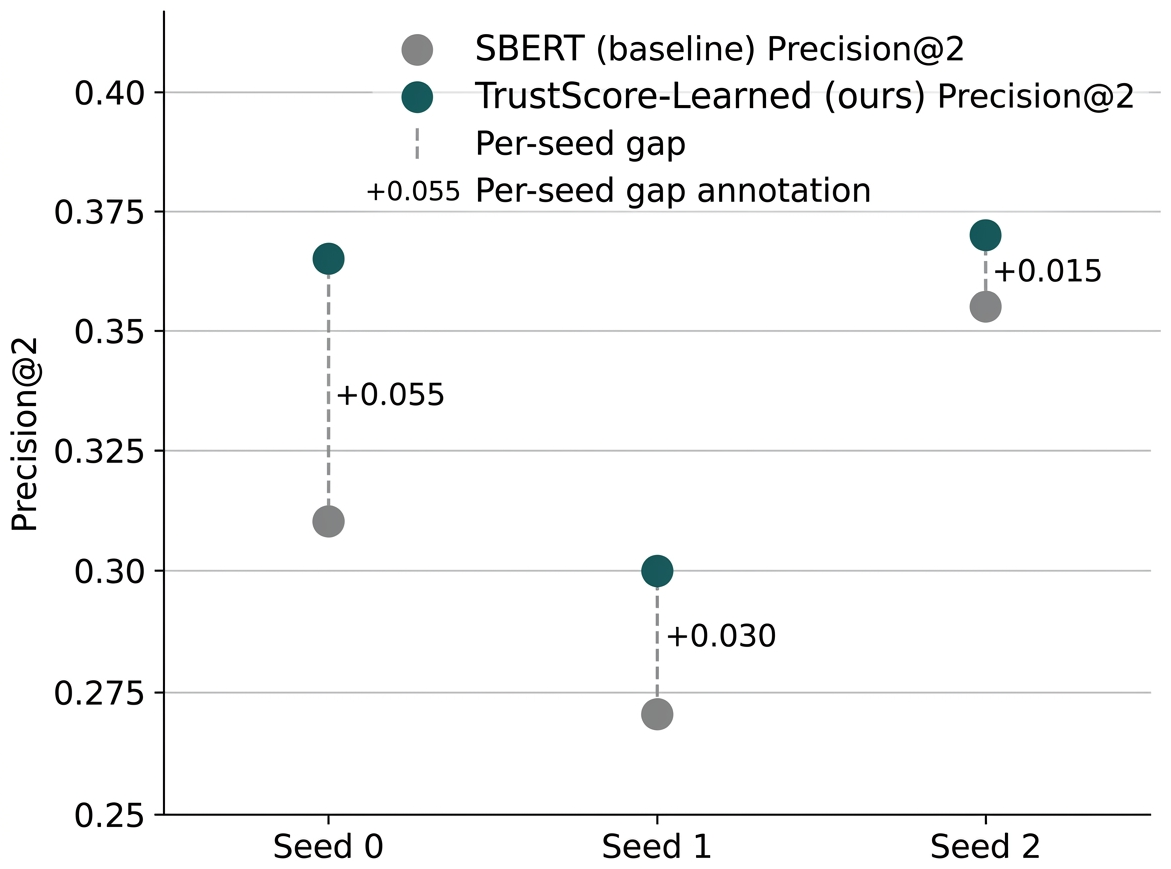
\includegraphics[width=0.95\linewidth]{figures/fig-per-seed.png}
  \caption{Per-seed Precision@2 for SBERT (grey) and Learned-TrustScore
  (dark teal) over three seeds. The gap is consistent in sign across
  all seeds: $+0.055$ (seed 0), $+0.030$ (seed 1), $+0.015$ (seed 2).}
  \label{fig:fig-per-seed}
\end{figure}

\subsection*{Ablation: uniform averaging of trust signals hurts}

The uniform-weight TrustScore, which averages three normalized
signals (SBERT relevance, log-paragraph-length as an authority proxy,
and mean cross-paragraph consistency), attains P@2 of only
$0.080 \pm 0.016$, below BM25 ($0.187$) and far below SBERT alone
($0.312$). Its paragraph F1 ($0.369$) and supporting-fact F1 ($0.174$)
are likewise the lowest among informed methods. This ablation isolates
the cause: combining trust signals without regard to their per-signal
calibration is actively harmful in distractor-rich retrieval, because
individual signals can be anti-correlated with ground truth.

\subsection*{Which signals help and which hurt?}

Table~\ref{tab:weights} reports the logistic-regression weights averaged
across seeds. The learned model assigns strongly positive weights to
semantic relevance (sbert\_rel, $+3.09 \pm 0.31$) and lexical relevance
(bm25, $+1.76 \pm 0.13$), and moderate positive weights to TF-IDF
($+0.64 \pm 0.18$) and the question-entity-overlap signal
($+0.62 \pm 0.18$). Critically, it assigns \emph{negative} weights to
paragraph log-length ($-0.98 \pm 0.37$) and cross-paragraph consistency
($-0.88 \pm 0.10$), identifying them as anti-signals in the HotpotQA
distractor setting. Two distinct mechanisms fit each negative weight:
(a) Wikipedia-sourced distractors and gold paragraphs share length
profiles, so length carries no discriminative authority signal; (b)
HotpotQA distractors are sampled to be topically close to the query,
inflating their cross-paragraph consistency above that of the true gold
pair. An uncritical application of textbook trust heuristics would
import these two features with positive sign; supervised calibration
over only 100 examples reverses them.

\begin{table}[!tbp]
\centering
\footnotesize
\setlength{\tabcolsep}{3pt}
\resizebox{\columnwidth}{!}{%
\begin{tabular}{@{}lc@{}}
\toprule
Feature & Learned weight (mean $\pm$ std) \\
\midrule
sbert\_rel (query-para.\ cosine) & $\mathbf{+3.09 \pm 0.31}$ \\
bm25                              & $\mathbf{+1.76 \pm 0.13}$ \\
tfidf                             & $+0.64 \pm 0.18$ \\
entity\_overlap (ours)            & $+0.62 \pm 0.18$ \\
log\_len (length proxy)           & $\mathbf{-0.98 \pm 0.37}$ \\
consistency (cross-source)        & $\mathbf{-0.88 \pm 0.10}$ \\
\bottomrule
\end{tabular}%
}
\caption{Mean logistic-regression weights for Learned-TrustScore across three seeds, 100 training questions per seed. Positive weights contribute toward ``gold''; negative weights are learned as anti-signals. Bolded rows have $|\bar w| > 0.8$ and consistent sign across every seed.}
\label{tab:weights}
\end{table}

\begin{figure}[!tbp]
  \centering
  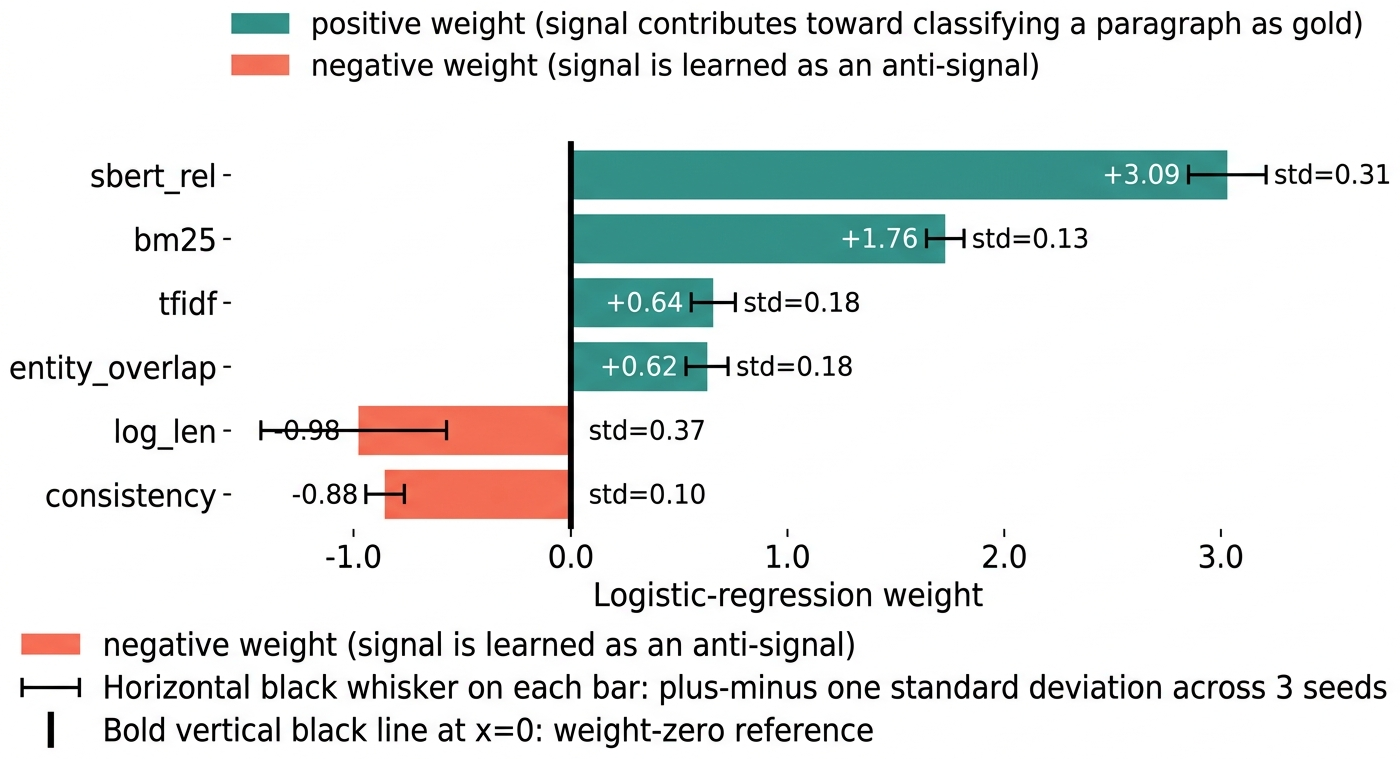
\includegraphics[width=0.95\linewidth]{figures/fig-weights.png}
  \caption{Fitted Learned-TrustScore weights, averaged across three
  seeds (error bars $\pm 1$ std). Positive weights (teal) contribute
  toward classifying a paragraph as gold; negative weights (coral) are
  learned as anti-signals. Paragraph length and cross-paragraph
  consistency flip negative.}
  \label{fig:fig-weights}
\end{figure}

\subsection*{Scope of the reported numbers}

All numbers in this section are computed on a 200-question held-out
subset per seed (600 distinct evaluations drawn from the 7{,}405
HotpotQA distractor validation questions). The margin over SBERT, while
per-seed consistent, is only slightly larger than a single seed-std;
larger-subset or larger-seed studies would tighten this bound. The
learned classifier is trained on 100 questions per seed, and the effect
of training budget on learned-trust calibration is not swept here. The
study characterizes retrieval-side selection only: downstream
question-answering accuracy with the selected paragraphs is deferred to
future work.
